\documentclass[
	classe=$2^{de}$,
	headerTitle=Activité,
	landscape,
	twocolumn
]{exercice}

\usepackage{tikz-repère}
\usetikzlibrary{calc}

\newdimen{\tempx}
\newdimen{\tempy}
\newcommand{\getx}[1]{
	\coordinate (tmp) at #1;
	\pgfextractx\tempx{\pgfpointanchor{tmp}{center}}
}
\newcommand{\gety}[1]{
	\coordinate (tmp) at #1;
	\pgfextracty\tempy{\pgfpointanchor{tmp}{center}}
}

\setlength{\columnsep}{1cm}

\begin{document}

\title{Activité : calcul de la norme}
\maketitle

\begin{center}
	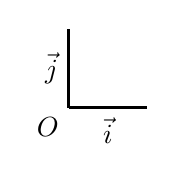
\begin{tikzpicture}
		\tikzRepere{-5.5}{5.5}{-3.5}{3.5}[][]

		\node[below left] at (0,0) {$O$};
		\draw[thick,\myArrow] (0,0) -- node[below] {$\vec{i}$} (1,0);
		\draw[thick,\myArrow] (0,0) -- node[left] {$\vec{j}$} (0,1);

		\ifdefined\makeCorrection
			\coordinate (A) at (4, 3);
			\coordinate (B) at (5, -1);
			\coordinate (C) at (-2, 1);
			\coordinate (D) at ($(B) + (C) - (A)$);
			\getx{(D)}
			\gety{(B)}
			\coordinate (E) at (\tempx,\tempy);


			\foreach \p in {A,B,C,D,E} {
					\node at (\p) {$×$};
					\node[below left] at (\p) {$\p$};
				}
		\fi
	\end{tikzpicture}
\end{center}

\begin{enumerate}
	\item Dans le repère orthonormé ci-dessus, placer les points $A(4 ; 3)$, $B(5 ; -1)$ et $C(-2 ; 1)$.
	\item Placer le point $D$ tel que $\vec{AB} = \vec{CD}$.
	\item Donner les coordonnées du vecteur $\vec{DB}\begin{pmatrix}\correction{6} \\ \correction{2} \end{pmatrix}$.
	\item Placer le point $E$, de sorte qu'il ait la même abscisse que $D$ et la même ordonnée que $B$.

	      Que peut-on alors dire du triangle $BDE$ ? \correction{Il est rectangle}
	\item Calculer la norme $‖\vec{DB}‖$ du vecteur $\vec{DB}$ (utiliser le théorème de Pythagore !). \correction{$‖\vec{DB}‖ = \sqrt{6² + 2²} = \sqrt{40}$}
\end{enumerate}

\newpage
\title{Activité : calcul de la norme (2)}
\maketitle

\begin{center}
	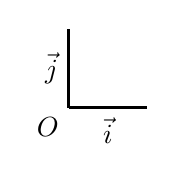
\begin{tikzpicture}
		\tikzRepere{-5.5}{5.5}{-5.5}{3.5}[][]

		\node[below left] at (0,0) {$O$};
		\draw[thick,\myArrow] (0,0) -- node[below] {$\vec{i}$} (1,0);
		\draw[thick,\myArrow] (0,0) -- node[left] {$\vec{j}$} (0,1);

		\ifdefined\makeCorrection
			\coordinate (A) at (-5, -2);
			\coordinate (B) at (-4, 3);
			\coordinate (C) at (-4, -5);
			\coordinate (D) at (3, -1);

			\foreach \p in {A,B,C,D} {
					\node at (\p) {$×$};
					\node[below left] at (\p) {$\p$};
				}
		\fi
	\end{tikzpicture}
\end{center}

\begin{enumerate}
	\item Placer dans le repère orthonormé ci-dessus les points $A(–5 ; –2)$, $B(–4 ; 3)$, $C(–4 ; –5)$ et $D(3 ; –1)$.
	\item Calculer les longueurs $DA$, $DB$ et $DC$. \correction{$DA = DB = DC = \sqrt{65}$}
	\item En déduire que les points $A$, $B$ et $C$ appartiennent à un même cercle dont on précisera le centre et le rayon. \correction{Cercle de centre $D$ et de rayon $\sqrt{65}$}
	\item Sans les placer, les points $E(10 ; 3)$ et $F(6 ; –7)$ appartiennent-ils aussi à ce cercle ? \correction{$DE = \sqrt{7² + 4²} = \sqrt{65}$ et $DF = \sqrt{3² + 6²} = \sqrt{45}$}
\end{enumerate}

\end{document}